%%%%%%%%%%%%%%%%%%%%%%%%%%%%%%%%%%%%%%%%%%%%%%%%%%%%%%%%%%%%%%%%%%%%%%
% amspaper.tex --  LaTeX-based template for submissions to American 
% Meteorological Society journals
%
% Template developed by Amy Hendrickson, 2013, TeXnology Inc., 
% amyh@texnology.com, http://www.texnology.com
% following earlier work by Brian Papa, American Meteorological Society
%
% Email questions to latex@ametsoc.org.
%
%%%%%%%%%%%%%%%%%%%%%%%%%%%%%%%%%%%%%%%%%%%%%%%%%%%%%%%%%%%%%%%%%%%%%
% PREAMBLE
%%%%%%%%%%%%%%%%%%%%%%%%%%%%%%%%%%%%%%%%%%%%%%%%%%%%%%%%%%%%%%%%%%%%%

%% Start with one of the following:
% DOUBLE-SPACED VERSION FOR SUBMISSION TO THE AMS
\documentclass{ametsoc}

% TWO-COLUMN JOURNAL PAGE LAYOUT---FOR AUTHOR USE ONLY
% \documentclass[twocol]{ametsoc}

%%%%%%%%%%%%%%%%%%%%%%%%%%%%%%%%
%%% To be entered only if twocol option is used

\journal{jcli}

\usepackage{color}

%  Please choose a journal abbreviation to use above from the following list:
% 
%   jamc     (Journal of Applied Meteorology and Climatology)
%   jtech     (Journal of Atmospheric and Oceanic Technology)
%   jhm      (Journal of Hydrometeorology)
%   jpo     (Journal of Physical Oceanography)
%   jas      (Journal of Atmospheric Sciences)	
%   jcli      (Journal of Climate)
%   mwr      (Monthly Weather Review)
%   wcas      (Weather, Climate, and Society)
%   waf       (Weather and Forecasting)
%   bams (Bulletin of the American Meteorological Society)
%   ei    (Earth Interactions)

%%%%%%%%%%%%%%%%%%%%%%%%%%%%%%%%
%Citations should be of the form ``author year''  not ``author, year''
\bibpunct{(}{)}{;}{a}{}{,}

%%%%%%%%%%%%%%%%%%%%%%%%%%%%%%%%

%%% To be entered by author:

%% May use \\ to break lines in title:

\title{Characterizing precipitation behaviors from recent historical climate to 21st Century over Western United States}

%change the title?

%%% Enter authors' names, as you see in this example:
%%% Use \correspondingauthor{} and \thanks{Current Affiliation:...}
%%% immediately following the appropriate author.
%%%
%%% Note that the \correspondingauthor{} command is NECESSARY.
%%% The \thanks{} commands are OPTIONAL.

    \authors{Xingying Huang, \correspondingauthor{Xingying Huang, 
     Department of Land, Air and Water Resources,
     University of California Davis, Davis, CA 95616.}
     Paul A. Ullrich}

     \affiliation{Department of Land, Air and Water Resources, University of California, Davis}

\email{xyhuang@ucdavis.edu}


    \extraauthor{}
    \extraaffil{}


%%%%%%%%%%%%%%%%%%%%%%%%%%%%%%%%%%%%%%%%%%%%%%%%%%%%%%%%%%%%%%%%%%%%%
% ABSTRACT
%
% Enter your Abstract here

\abstract{} 


\begin{document}


%% Necessary!
\maketitle


%%%%%%%%%%%%%%%%%%%%%%%%%%%%%%%%%%%%%%%%%%%%%%%%%%%%%%%%%%%%%%%%%%%%%
% MAIN BODY OF PAPER
%%%%%%%%%%%%%%%%%%%%%%%%%%%%%%%%%%%%%%%%%%%%%%%%%%%%%%%%%%%%%%%%%%%%%
%
\section{Introduction}

Precipitation changes have always been an important issue that bring a lot attention in climate modeling studies, due to the significant impacts of precipitation related phenomenon especially for drought occurrence and heavy precipitation events \citep{seneviratne2012changes}. There are a number of studies aiming to find out how the precipitation will behave in future based on varied climate forcing scenarios under anthropogenic-induced changes \citep{hegerl2004detectability, kharin2007changes, scoccimarro2013heavy}, stating that the world is getting wetter relating with a warmer climate. However, the impacts of climate change vary regionally in their severity, with more attention need to be paid on regional climate extremes study to make effective responses. 

%Changes in rainfall distributions have attracted much attention because of the particular vulnerability of human activities to hydrological extreme events such as flood-producing rains and droughts. 
%The intensity of extreme precipitation is projected to increase under global warming in many parts of the world, even in the regions where mean precipitation decreases

%Extreme temperatures and heavy precipitation have significant impacts to both our socioeconomic and natural systems. Globally, heat extremes have been increasing, with reducing extreme low temperatures

%


Although prediction of future climate has large uncertainty, climate model simulations are nonetheless the most useful information we can resort to study potential climate variability and extremes changes in future \citep{easterling2000climate}. Global climate models (GCMs) are primarily used to investigate possible future changes in mean climate mean, variability and extremes, forced with projected greenhouse gas concentration and aerosol emissions. There are a large amount studies and results concerning the global changes of climate extremes \citep{seneviratne2012changes}, but much less efforts focusing on the regional scale which is needed in order to implement climate adaptation and mitigation strategies. Due to the coarse resolutions ($\sim$1$^\circ$) of GCMs, regional climate models (RCMs) are mostly used to get the frequency, intensity, and duration of extreme events, by better capturing fine-scale dynamical features with high horizontal resolution \citep{bell2004regional, frei2006future, rauscher2010resolution, wehner2013very}. Higher resolution can allow better simulation of precipitation extremes, related with regional representation in land use, land�water contrast, snow cover, cloudiness and circulation patterns associated with fine topography \citep{leung2003regional, diffenbaugh2005fine, salathe2008high, wehner2010effect}. 

%*** \citep{mass2011extreme} this paper has detailed discussion of precipitation extremes over western US modeled by other studies. (see the last two paragraphs)

%%wehner2013very   Very extreme seasonal precipitation in the NARCCAP ensemble: model performance and projections
%wehner2010effect  The effect of horizontal resolution on simulation of very extreme US precipitation events in a global atmosphere model
%rauscher2010resolution  Resolution effects on regional climate model simulations of seasonal precipitation over Europe

%***singh2013precipitation  Precipitation extremes over the continental United States in a transient, high-resolution, ensemble climate model experiment see the plots
%frei2006future   Future change of precipitation extremes in Europe: Intercomparison of scenarios from regional climate models 

%***\cite{diffenbaugh2005fine} studied both hot and wet events over the contiguous United States based on RCMs simulation at 25km horizontal resolution, showing that fine-scale processes are critical for accurate assessment of local and regional scale vulnerability to climate change. However, it does not mean that higher resolution can always perform better, and this aspect will be investigated in our study through multi-scale simulations including ~10km horizontal resolution.

%***"Simulations with global coupled ocean�atmosphere general circulation models (CGCMs) forced with projected greenhouse gas and aerosol emissions are the primary tools for studying possible future changes in climate mean, variability, and extremes. Changes in rainfall distributions have attracted much attention because of the particular vulnerability of human activities to hydrological extreme events such as flood-producing rains and droughts. The intensity of extreme precipitation is projected to increase under global warming in many parts of the world, even in the regions where mean precipitation decreases" \citep{kharin2007changes}

%***"climate model improvements have resulted in an enhanced ability to simulate many aspects of climate variability and extremes. However, they are still characterized by systematic errors and limitations in accurately simulating regional climate conditions." \citep{easterling2000climate}

%Leung and Qian (2003) showed that the higher-resolution nest yields more realistic precipitation patterns and produces more frequent heavy precipitation, which is consistent with observations.


Except RCMs, variable-resolution enabled GCMs (VRGCMs) are also one of the dynamical downscaling methods that has been receiving a growing interest in modeling regional climate recently. Unlike RCMs, which are forced by the output from GCMs for future projections, VRGCMs use a relatively coarse global model with enhanced resolution over a specific region \citep{staniforth1978variable, fox1997finite}, demonstrating utility for regional climate studies and applications at a reduced computational cost compared to uniform-resolution GCMs \citep{fox2006variable, rauscher2013exploring}. Contrasted with RCMs, VRGCMs use a single, unified modeling framework rather than two separate models (GCM and RCM) with potentially disparate dynamics and physics parameterizations, avoiding the inconsistencies and lack of two-way interactions between the global and regional scales at the nest boundary of RCMs \citep{mcdonald2003transparent, laprise2008challenging, mesinger2013limited}. 

For our purpose, we use the recently developed variable-resolution option in Community Earth System Model (VR-CESM) to get the potential changes of precipitation extremes till end of 21st century over western U.S. For decades, CESM (and its predecessor, the Community Climate System Model) has been used for modeling present and future global climate \citep{neale2010description, hurrell2013community}. The overall performance of VR-CESM in modeling California�s climate has been addressed in detail in \cite{huang2016evaluation}, which demonstrates VR-CESM has competitive biases when compared with a regional climate model forced by reanalysis data, as evaluated against high-quality observations and reanalysis datasets. VR-CESM has also been employed by other studies showing the comparable ability in capturing fine-scale atmospheric processes as uniform CESM or a RCM, and do not exhibit apparent artifacts in the variable-resolution transition region \citep{rhoades2015characterizing, zarzycki2014using, zarzycki2015effects}.

%In our study, and previous studies (e.g. \cite{zarzycki2015effects}), general circulation patterns (e.g., wind, pressure and precipitation) do not exhibit apparent artifacts in the variable-resolution transition region, and the design of the SE dynamical core ensures that dry air and tracer mass are conserved globally \citep{taylor2010compatible}.

%statistical downscaling

%\cite{rhoades2015characterizing} has also assessed the promising use of VR-CESM for modeling Sierra Nevada mountain snowpack in the western United States. Variable resolution has also been employed by \cite{zarzycki2014using} to show that a high-resolution refinement patch in the Atlantic basin for simulating tropical cyclones represented significant improvements over the unrefined simulation. \cite{zarzycki2015effects} have compared the large-scale climatology of VR-CESM 0.25$^\circ$ and uniform CESM at 1$^\circ$, evaluated with reanalysis (MERRA, NCEP) dataset, and found that adding a refined region over the globe did not significantly affect the global circulation. In our study, as in \cite{zarzycki2015effects}, general circulation patterns (e.g., wind, pressure and precipitation) do not exhibit apparent artifacts in the variable-resolution transition region, and the design of the SE dynamical core ensures that dry air and tracer mass are conserved globally \citep{dennis2011cam, taylor2010compatible, taylor2011conservation}.


%VR-CESM is driven by the Community Atmosphere Model's (CAM's) Spectral Element (SE) dynamical core, which possesses attractive conservation and parallel scaling properties \citep{dennis2011cam, taylor2011conservation}, as well as recently developed variable-resolution capabilities \citep{zarzycki2014aquaplanet, zarzycki2015experimental}. 


Overall, in this paper, we focus on investigate the changes of precipitation behaviors during 21st Century over western U.S. based on long-term ensemble runs conducted by VR-CESM at the resolution of 0.25$^\circ$. Simulations are performed following the RCP (reference concentration pathways) 8.5 scenario, representing the highest rate of increase in greenhouse gas concentrations within the new set of RCPs. We anticipate to obtain the changes of overall precipitation and the upper bound of the precipitation events distribution under warmer climate with high-resolution simulation output from the recent-climate to the end of 21st Century. This study aims to further improve our understanding of both past and future regional precipitation behaviors at fine-scale. {\color{red}(add more text here)}

%***Over western U.S. heat and precipitation extremes show increasing trend in different subregion \citep{duffy2006simulations}. "Simulations of present and future climates in the western United States with four nested regional climate models"
%***\citep{duliere2011extreme} "Extreme Precipitation and Temperature over the US Pacific Northwest: A Comparison between Observations, Reanalysis Data, and Regional Models*"
%***\citep{salathe2008high} "A High-Resolution Climate Model for the US Pacific Northwest: Mesoscale Feedbacks and Local Responses to Climate Change*"

This paper is structured as following. Section 2 describes the model setup, methodology and reference datasets used. Results are presented and analyzed in Section 3 including the model evaluation, mean climatology trend and precipitation extremes changes. Section 4 summarizes the main points of the study along with detailed discussion.


(add the hypothesis we want to argue here) (a) the choice of index b) the use of VR-CESM c) study of the ENSO and climate forcing together)

%jaeger2011impact,  Impact of soil moisture--atmosphere coupling on European climate extremes and trends in a regional climate model

%Kenyon, Jesse, and Gabriele C. Hegerl. "Influence of modes of climate variability on global temperature extremes." Journal of Climate 21.15 (2008): 3872-3889.

%*** refer paper: for impacts of extreme events (definition and also use EVA method to get return level) \citep{mastrandrea2011current} Current and future impacts of extreme events in California

%pierce2013probabilistic   Probabilistic estimates of future changes in California temperature and precipitation using statistical and dynamical downscaling
%cooley2007bayesian  Bayesian spatial modeling of extreme precipitation return levels  
%cooley2010spatial  Spatial hierarchical modeling of precipitation extremes from a regional climate model
%\citep{schliep2010comparison}  "A comparison study of extreme precipitation from six different regional climate models via spatial hierarchical modeling"

\section{Models and Methodology}

\subsection{Model setup}

As above-mentioned, CESM, as a state-of-the-art Earth modeling framework, consists of coupled atmospheric, oceanic, land and sea ice models \citep{CAM5Tech, hurrell2013community}. In this study, Community Atmosphere Model version 5 (CAM5) \citep{CAM5Tech} and the Community Land Model version 4.0 \citep{CLM40Tech} are used. CAM 5 is driven by the Spectral Element (SE) dynamical core with conservation and parallel scaling properties \citep{dennis2011cam, taylor2011conservation} and supporting variable-resolution option \citep{zarzycki2014using}. Global sea-surface temperatures and sea ice are prescribed in accordance with the Atmospheric Model Intercomparison Project (AMIP) protocol \citep{Gates1992}, which are widely used and support climate model diagnosis, validation and intercomparison. The finest horizontal resolution of our grid is $\sim$28 km covering the western U.S., with a quasi-uniform 1$^\circ$ mesh over the remainder of the globe (See Figure \ref{fig:Figure 1}). A detailed description of the techniques of VR-CESM employed in this paper including the grids generation, topography preparation and component set can be found in \cite{rhoades2015characterizing, huang2016evaluation}. 

%***The coupling infrastructure in CESM communicates the interfacial states and fluxes between each component model to ensure conservation. Since we follow AMIP protocols, only the atmosphere and land model are integrated dynamically. The FAMIPC5 (F$\_$AMIP$\_$CAM5) component set, which mainly supports atmospheric, oceanic, land and sea ice models, is chosen for these simulations. In CAM5, cloud microphysics is parameterized using the two-moment scheme with with ice supersaturation \citep{ morrison2008new, gettelman2008new}, and the deep convection process is treated by Zhang and McFarlane (ZM) cumulus scheme \citep{zhang1995sensitivity}. A more detailed discussion of the CAM5 configuration can be found in \citet{neale2010description}.


Simulations have been conducted for both historical climate and transient future projections . The historical climate simulation cover the period 1979 through 2005. The transient future projections cover two periods including near future 2024-2050 and late-century 2069�2095. For purposes of analysis, the first year of each time period was discarded as a spin-up period to allow adequate time for the initialized land and atmosphere to equilibrate. The 26-year duration was chosen to provide an adequate sampling of annual variability for each time phase. For future projections, GHG concentrations are set based on RCP 8.5 senario which describes GHG emissions continue to rise throughout the 21st century \citep{riahi2011rcp}. Simulations are forced by observed sea-surface temperatures (SSTs) and sea ice for historical period at 1$^\circ$ as described by \citet{hurrell2008new}, and simulated SSTs and sea ice for future projections are provided by Hannay {\color{red} (add citation)}, without the added complexity of ocean-atmosphere feedbacks in the climate system. Land surface datasets, including plant functional types, at $0.5$$^\circ$ were adopted for each year.

%SST file: /glade/p/cesm/cseg/inputdata/atm/cam/sst

%In particular, observed SSTs and sea ice at 1$^\circ$ horizontal resolution are provided and updated following the procedure described by \citet{hurrell2008new}.

%*** The first of these (1981-2010) represents the reference period for model evaluation and for the calculation of climate changes.


Due to the uncertainty in future climate projections, ensemble simulations are needed, especially for climatology statistics associated with temperature and precipitations. However, due to the diverse internal variability for different climate models and for different climate variables, there is no standard criteria for the minimum number of simulations needed for climate extremes studies \citep{deser2012uncertainty}. According to Ryan L. Sriver et al. (2014) {\color{red}(add citation)}, CESM ensemble show obviously smaller uncertainty than Coupled Model Intercomparison Project Phase (CMIP) 5 for both temperature and precipitation in North America. Based on the results of \cite{deser2012uncertainty}, at least three ensemble runs are required to detect a significant epoch difference for the JJA surface temperature, and for precipitation, more than 40 ensemble runs are needed. Considering that we did not explicitly use coupled ocean model and we focused on regional area at much finer resolution, in this study, we did four simulations for each future time period. We also have two runs for the historical period. Due to the relatively small uncertainty within the runs over the same time period (shown by the supplement), we assume that the numbers of ensemble runs applied in this study are enough to satisfy our goal. 

{\color{red}plot in supplement: the relative difference between specific run and ensemble mean of different period}



%***The use of an ensemble of simulations is particularly useful for also determining the statistics of the climatology generated in each case, including the mean and variance associated with each of the variables of interest.

%*** Actually, former studies of regional high-resolution climate extremes usually use no more than five members \citep{diffenbaugh2010intensification}. We will analyze the uncertainty among multi-scale simulations for heat and precipitation extremes distribution. We may increase the ensemble members if needed and computation resources allowed.

%multi-member ensemble simulations provide additional insight into sources of uncertainty within a model simulation (Rougier et al. 2009; Flato et al. 2013).

%GCM: meehl2004more use four for past, five for future; VRGCM with one simulation seem ok for past climate; based on sriver_ppt_Analyzing climate impacts using a low resolution CESM ensemble, pg18, five ensemble should be ok for heat extremes, but not enough for precipitation extremes, one VRGCM should be ok for mean climate.

%Richard: In fact, if you are doing 1 model run for historical simulations and only 5 for future climate, it is very unlikely you will have any unambiguous results. An example reference might be Deser et al, 2012, Nature Climate Change. Wallace, Fischer, Thompson, and Deser discussed this at length in their 4 separate talks at AGU last month. Deser has another paper which looks at numbers of model runs or time periods or similar needed and it is different for max T than for precipitation.

%*** Omitting the coupled ocean model saves considerable computation and allows the atmospheric model to be run at higher resolution


\section{Methodology}

%In order to catch the hot spells, we used the daily maximum temperature (Tmax) data from May 1st to September 30th over our simulation period. Two main approaches are applied to characterize the behavior of hot spell. One is the extreme indexes method. We have tested different indexes and exhibited the most useful ones in this paper, as Table showed. We have used both 90\% and 95\% percentile of each grid point over whole dataset as the thresholds to define the hot spells and extreme hot spells. In oder to account for how hot it really feels to the human body, relative humidity is combined with the dry air temperature to get the heat index (i.e. the apparent temperature). Heat index is defined in Equation (insert Equation). When capturing the hot spell, declustering is considered to make sure the data are serially independent of one another based on the schemes provided by Ferro and Segers (2003) \citep{ferro2003inference}, which is included in the R packaged extReme (add citation here). \cite{coles2001introduction} gave a discussion of the need to decluster and the modeling of extremes of dependent series in general.

%And we have tested that the 5\% upper tail values of annual datasets almost all fall in this time period. 
%A more general view on declustering schemes was provided by Ferro & Segers (2003). (Furrer et al. 2010)
%decluster interval function: ferro2003inference (seems complicated, also see the R help of decluster); extreme index close to 1 (this value is in the decluster return variable)


%Simulation output will be analyzed to get the return level of the heat extremes by using the method of EVA for stationary extremes (i.e. unchanging climate). Specifically, we used the peaks-over-threshold (POT) modeling of threshold excesses using the generalized GP distribution (insert Equation) due to its advantages in describing climatic extreme values \citep{brown2008global, furrer2010statistical}. And using POT modeling approach, more sample can be utilized than a block maximum approach. The R package \texttt{extRemes} has been applied to assist POT modeling. Data exceeding a predefined threshold has been analyzed and the threshold values are also determined using 90\% percentile of each grid point as the one used in indexes analysis. L-moments is used as the parameter estimation method since it required less computational effort compared to other traditional techniques, such as Maximum likelihood (ML) and Bayesian, and it has better sampling properties than ML or the method of conventional moments \citep{zwiers1998changes, fruh2010determination}. Hosking and Wallis (1997) (add citation here) showed that L-moments are efficient in estimating parameters of a wide range of distributions from small samples. (Fr�h et al. 2010) (add citation here). The goodness-of-fit of the fitted distribution has been done with Kolmogorov-Smirnov (K-S) test, and the data fit the GP distribution.

%to do: test: GP with Bayesian, PP with MLE and Bayesian
%to do: testify stationary extremes (i.e. unchanging climate)
%the uncertainty of the distribution�s parameters will be evaluated by confidence intervals for return level estimation.

%Heidke skill score
%EOF analysis
 
%PP: which fitting the GP df to excesses over a high threshold and also estimating the frequency of exceeding the threshold by fitting a Poisson distribution
%The point process approach has several advantages over the block maxima and the POT approaches: (1) it uses considerably more data about extremes than a block maximum approach, resulting in more reliable results; (2) it can be formulated in terms of the GEV parameters, which are invariant to the choice of threshold, allowing non-stationarities such as trends to be easily and naturally introduced through covariate effects in the parameters; and (3) it includes the threshold excess rate in the inference, which is modeled separately in a POT approach. Note that parameter estimation via maximum likelihood requires specialized but straightforward numerical techniques in the nonstationary case. (Furrer et al. 2010)

%ML is preferred due to its ability in incorporating linear trend in the parameter. Since the L-moment ((Fr�h et al. 2010)) estimators show better skill for small samples \citep{fruh2010determination}, it might be tried if the sample size is insufficient to use ML. Also, the Bayesian prior distribution \citep{frei2006future, martins2000generalized} may be used to improve the robustness of maximum likelihood estimates. 

%non-stationary
%where the covariate t  is the date during the observational period scaled to range from 0 to 1. More complex time dependence was not investigated as linear forms are deemed an adequate first-order approximation to any nonstationarity and avoid finding nonlinearity that is just a product of natural internal climate variability. Furthermore the observational period is relatively short so there is a danger of over fitting if more complex time dependence is introduced. Applying this approach to future projections of climate may require more sophisticated covariates, such as global mean temperature, as future temperature changes are unlikely to be linear [Cubasch et al. , 2001]. The inclusion of NAO as a covariate is described later. (Brown, Caesar, and Ferro 2008)


In order to thoroughly capture the frequency, intensity, and duration of precipitation events distribution at each time period, we used all the daily precipitation data of our simulations since strong precipitation events can occur in different seasons for diverse climate divisions. As a common approach, extreme indices are employed to depict the behaviors of precipitation \citep{tebaldi2006going, zhang2010influence, duliere2011extreme, zhang2011indices, sillmann2013climate}. In our study, we have tried many relevant indices including those defined by the Expert Team on Climate Change Detection and Indices (ETCCDI) and others used in previous studies depicting the percentiles, maximum value, or the events changes of Pr. It turned out that those are suitable for our purpose here, since we assume that the indices used should be suitable, easily interpreted and being relevant for policy makers. Therefore, we end up with the indices summarized in Table \ref{tab:table1} defining the different ranges of precipitation distributions.

%In this study, we have used selected indices in previous studies  \citep{tebaldi2006going, zhang2010influence, duliere2011extreme, zhang2011indices, sillmann2013climate} and also defined other indices that are suitable, well interpreted and describe extremes in a comprehensive and objective way. 
%(Before using indices method for extreme analysis, we need to select indices which are suitable, as easy as possible to be interpreted, being relevant for policy makers and describe extreme processes in a comprehensive and objective way \citep{sanchez2004future}.)

%**** The indices we used are summarized in Table \ref{tab:Table1} {\color{red}add table 1 based on $pr_extreme_Hist_2runs.pdf$}. We can divide the indices into two types. One kind is to describe the overall features of precipitation including the {\color{red} to be added}. The other kind is to define precipitation events, using specific rain rates of 1mm, 10 mm, 20 mm, 30mm, 40 mm and 50 mm as the thresholds. Specifically, a event is captured at each grid cell with consecutive days of rain rate exceeding corresponding threshold. A dry event is defined similarly except that it is the days without rain (Pr<=1.0mm/day). When capturing wet events, rainy days with precipitation rate less than the specific threshold are not treated as gap for different spells, and are surely not included in the wet event's duration length. 

%*** The indices are loosed based on the ones defined by the Expert Team on Climate Change Detection and Indices (ETCCDI), which have been widely accepted and applied.

%*** focusing on describing features in the tails of data distributions. Indices have been commonly used for a long time, and have contributed a lot to climate analyses on extremes \citep{zhang2011indices} 
%and percentiles of 90\% and 95\% of each grid point over all rainy days, 

%zhang2011indices  Indices for monitoring changes in extremes based on daily temperature and precipitation data

%There are generally two approaches used in temperature and precipitation extremes analysis. One is the commonly used extreme indices \citep{tebaldi2006going, zhang2010influence, duliere2011extreme}. Another method is called extreme value analysis (EVA), using statistical model to characterizing extreme values \citep{coles2001introduction}. Though EVA method has also been shown to adequately capture the behavior of heat or precipitation extremes\citep{kharin2000changes, kharin2005estimating, furrer2010statistical,  photiadou2014modeling}, the use of this method still remains arguable within the climate research community \citep{katz2010statistics}. In our study, the two methods will be combined with necessary modifications to analyze the heat and precipitation extremes more comprehensively. And we will see if EVA method can bring important complementary information than just using extreme indices approach. This may bring us a wider view in extremes studying.


Due to the important role ENSO plays in regulating the precipitation over southwest U.S. (add citation here zhang2010influence, deser2012communication), the phase of ENSO (El Nino and La Nina) over each year is identified by the Nino 3.4 index. Some papers discuss that Nino 3.4 can not capture ENSO well, like \cite{kao2009contrasting}, we tried to widen the location (from 170W to 105W rather than from 170W to 120W ) a little bit, the SST anomaly of each year is quite similar to what we got from Nino 3.4, especially for future periods. Therefore, we presume it won't really affect our results whether the location extends or not.

%linear regression is applied to signaling the factor effects due to ENSO and climate forcing. Firstly, we get the phase of ENSO over each year including El Nino, La Nina and normal state at each grid point over our study area followed by the way of ENSO 3.4 (add citation here) (add more details about how ENSO is calculated over each time period). Next, we naturally divide climate forcing into three scenarios represented by each time period. The features of wet or dry spell as we described above are used as response variable. Mathematically, the regression relationship can be written as, (add equation and explain it here).

(The values of Nino index: see supplement. $indices\_oni.pdf$ (update this figure))

%%%ENSO 3.4 using SST dataset define the baseline http://www.cpc.ncep.noaa.gov/products/analysis_monitoring/ensostuff/ONI_change.shtml

%{ropelewski1986north} "North American precipitation and temperature patterns associated with the El Ni�o/Southern Oscillation (ENSO)."  
%{cayan1993nino} "El Ni{\~n}o/southern oscillation and streamflow in the western United States"

%(fulfill the model assumption (p-norm) and the sizes should be enough)

%****Throughout the remainder of this paper, Student's t-test has been used to test whether two sets of dataset at each grid point or spatially averaged over specific climate division are the same, when the sample population can be adequately described by a normal distribution. The normality of a dataset is assessed under the Anderson-Darling test. When the sample populations do not approximately follow a normal distribution, Mann-Whitney-Wilcoxon (MWW) test is employed in lieu of the t-test. All these tests are evaluated at the $\alpha = 0.05$ significance level.

%statistical significance for necessary variables: note the ad.test is based on sample size >7, therefore, this does not fit for extreme events that happen too less, combined all ensembles to get enough sample size


{\color{red}(add description of the supplement)}

%may to be added: spatial division, return level, SPI or PDSI

%The uncertainty of average precipitation within ensemble runs is quite small.

%Return levels of the wet extremes are also retrieved by using the method of EVA for stationary extremes. {"Specifically, we used the peaks-over-threshold (POT) modeling of threshold excesses using the generalized GP distribution (insert Equation) due to its advantages in describing climatic extreme values \citep{brown2008global, furrer2010statistical}. Data exceeding a predefined threshold has been analyzed and the threshold values are also determined using 90\% percentile of each grid point as the one used in indexes analysis. The goodness-of-fit of the fitted distribution has been done with Kolmogorov-Smirnov (K-S) test, and the data fit the GP distribution." these sentences to be changed accordingly}

%Similar as hot spell analysis, both indexes method and EVA method are applied to characterize the behavior of wet or dry spell. 

% one day gap for declustering dataset  rain gap for wet spell

%The future projections simulations will be analyzed to get the trend of the anthropogenic influences (changing of GHG) on these extremes. Overall, simulation output from varres-CESM will be analyzed to get the frequency, intensity, duration and return level of the heat and precipitation extremes by combined methods of indices and EVA, and evaluated by a variety of reference datasets.

\subsection{Reference datasets}

UW, CPC, NARR%, ASD

(add the descriptions of these datasets here)

%ASD:  (�The high-resolution CESM was run under �present-day� (year 2000) greenhouse gas conditions (fixed CO2 concentration of 367 ppm). This was chosen so that direct comparisons could be made with recent-era observations of fine-scale and large-scale phenomena.�)  https://www.earthsystemgrid.org/home.html

%PRISM (too fine), CFSR (at 0.5degree, so does not fit here)

%PRISM: tried plot Tmax PDF over CV, the shape is strange and quite different from UW.

%CFSR 0.3 deg: reanalysis dataset. Tmax and Tmin is 6 hourly forecast, Rh is 6 hourly forecast at 0.5 degree (I interpolated it to 0.3 deg). These are not forecast datasets rather than reanalysis datasets. ???


\section{results}


\subsection{evaluation}


%mean precipitation, SDII, days when daily pr is between (1, 5) (5, 10) (10, 20) (20, 40) >40, and corresponding fraction of total pr

%see $hist\_ref\_evaluation.pdf$

%***(add CESM ensemble at 1degree at the supplement, see the directory of discussion)
%***(percentile and event number etc. in $index1\_ref\&hist.pdf$ (from v4) can be put in the supplement, the new features from v5 can also be added in the supplement)

In order to see whether the model can capture the mean features of precipitation distribution, the results from VR-CESM and references are shown in Figure \ref{fig:Figure 2} including the mean precipitation and related indices. The fractions of rain amount for total Pr attributed by corresponding indices are also added in this figure to figure out the contribution of water of different ranges of Pr intensity. It can be seen that compared to observations, VR-CESM can well reproduce the spatial patterns of precipitation with quite similar magnitude, considering the uncertainty within these references. We also notice that CESM tends to overestimate the precipitation over the eastern side of the Cascades and the northern western side of the Sierra Nevada and overestimate the precipitation over the part of the Great Plains and the New Mexico, for precipitation rate under 20 mm/day. Biases in simulating extreme precipitation over the topographically complex regions have  been found \cite{singh2013precipitation}, being attributed to excessively strong winds. Most of the rain over dry area is obtained from non-extreme Pr (with Pr$=<$10mm), wile most of the precipitation over wet area is from extreme Pr (when Pr$>$10mm).


% VR-CESM close to UW 
%the 40-ensemble CESM runs: http://www2.cesm.ucar.edu/models/experiments/LENS Use the ensemble to further prove the need of fine resolution, and the reduce of uncertainty when resolution goes up
%�When presenting results based on the CESM Large Ensemble either in oral or written form, please acknowledge the CESM Large Ensemble Community Project and supercomputing resources provided by NSF/CISL/Yellowstone. An overview paper of the Large Ensemble Project should be cited as follows:
%�Kay, J. E., Deser, C., Phillips, A., Mai, A., Hannay, C., Strand, G., Arblaster, J., Bates, S., Danabasoglu, G., Edwards, J., Holland, M. Kushner, P., Lamarque, J.-F., Lawrence, D., Lindsay, K., Middleton, A., Munoz, E., Neale, R., Oleson, K., Polvani, L., and M. Vertenstein (2015), The Community Earth System Model (CESM) Large Ensemble Project: A Community Resource for Studying Climate Change in the Presence of Internal Climate Variability, Bulletin of the American Meteorological Society, doi: 10.1175/BAMS-D-13-00255.1, in press,�http://journals.ametsoc.org/doi/abs/10.1175/BAMS-D-13-00255.1�


\subsection{mean climatology}

Before getting into the analysis of the changes of precipitation features, it is important to understand the overall mean changes of precipitation and other relevant background variables. Since majority of the precipitation is from rainy seasons overing October to March (see Pr\_monthly.pdf in the supplement), Pr from each time period is depicted in each half of the year including the wet season from October to March and the dry season from April to September as we defined (see Figure \ref{fig:Figure 3}). 

Though temperature increases along with enhanced GHGs concentration, mean precipitation did not show notable changes. Mean precipitation tends to increase lightly over the northern western U.S during wet season, and over the central and southern part of WUS during dry season. There is a minor decrease of total precipitation over the Cascades and its western side during dry season, and also a light decrease of overall precipitation over part of the Sierra Nevada. No significant trend is observed for mean precipitation within each time period. 

As mean temperature goes up, there is consistent increase of 2m relative humidity over coastal region and west side of the Sierra Nevada in future, and slight decrease over most of the region during wet seasons. For dry seasons, the 2m relative humidity has slight increase over central-southern part of WUS during mid-century, and overall decrease over the remaining study area, especially during end-century. As argued by \cite{joshi2008mechanisms}, water vapor content over land does not increase fast enough relative to the rapid warming so that relative humidity will decrease on average, as also seen in other model simulations \citep{rowell2006causes} and observed on all continents \citep{simmons2010low}.

(update $pr\_mean\_clm.pdf$ using all the runs)

%(About the dryness of the surface/underground and relative humidity)
%"The key factor causing drying is that land surfaces (and the air just above them) warm, on average, about 50$\%$ more than ocean surfaces \citep{joshi2008mechanisms}" "The second factor ensuring drying is that water vapor content over land does not increase fast enough relative to the rapid warming there." "Because the land warms faster than the oceans, however, the humidity of the arriving air does not increase enough to maintain a constant relative humidity. The latter must therefore fall on average (see the figure), as indeed seen in model simulations \citep{rowell2006causes} and observed on all continents \citep{simmons2010low}." "In a warmer climate, more rain is needed. Many regions will get more rain, but it appears that few will get enough to keep pace with the growing evaporative demand."



%The moisture flux at 850 hPa (horizontal transport of water vapor by the wind) (seems to be consistent with the changes of relative humidity) (how to interpret this?)

%Figure: mean over each time period, PRECT, PRECC, and PRECL, T2avg, 2m relative humidity, moisture flux at 850 hpa.  see $pr_mean_clm.pdf$

%Almost all of the precipitation is resulted from large-scale meteorological processes rather than convection processes, except the west-central regions of WUS during hot seasons. 

%so most of the Pr comes from PRECL, except the westCentral regions of WUS during hot season
% Pr: different ensembles are quite similar

%wd_trend.pdf

%the low level cloud is kind of interesting as shown in the pg. 3 of Pr_dry_rain_season.pdf, though not sure how to explain it.
%% check if yearly trend exists: there is no significant linear trend no matter for annual pr, or dry season, wet season cesm_25_wd_index_trendtest.nc
%% most of the pr extreme days is during rainy season
%Tavg: the change of different ensemble: no notable difference

%***(add the uncertainty among different runs for those quantities in the supplement)

\subsection{Precipitation}

Given continuously increases of temperature in future, here the changes of precipitation features are displayed in Figure \ref{fig:Figure 4} including the differences between historical time period and future. It can be seen that precipitation distribution shows consistent trend of changes when going into mid of 21st century and till end of 21st century. The overall rainy days and frequency of non-extreme precipitation (i.e. with daily Pr no large than10 mm) have decreased lightly over the northern western U.S and California, and increased over the central and southern part of WUS, and this feature is mainly caused by the changes over dry seasons. As for the extreme precipitation frequency (i.e. with daily Pr between 10 mm and 40 mm), there is a decreasing trend over the Cascades and part of the Sierra Nevada, and a more obvious increasing trend over the northern western coast and eastern side of the Cascades. For the very extreme precipitation events, there is a notable increasing trend over the northern western coast and the Cascades, and a slight decrease over part of the Sierra Nevada. The decrease of rainy days during hot and dry season over central southern California, though with a minor magnitude, will probably intensify the drought condition due to the deficit of soil moisture due to higher evaportranspiration caused by the warmer climate in the future, as also found by \cite{cayan2010future, bell2004regional}.

(update the figures in discussion.pdf, add ivt and iwv when daily 40 mm$>= pr >$ 20 mm  and when pr $>$ 40 mm; might add the Z500 contour to the plot or Sea level pressure) add descriptions here. 

%(The projected changes are mainly associated with increases in the cold season water vapor influx from the Pacific Ocean.) \citep{diffenbaugh2005fine} "Radiative forcing and Enhanced low- and upper-level cyclonic flow" (Fig. 3. shows similar results to ours) ) (So the moisture supply for moderate or heavy precipitation locally does not come directly from evaporation. Instead it has to come from transport, and thus from convergence of low-level moisture elsewhere in the atmosphere. \citep{trenberth2003changing})

In order to investigate the impacts of large scale variability by ENSO, the difference of precipitation behaviors between the warm phase (i.e. El Nino) and cool phase (i.e. La Nina) of ENSO is illustrated in Figure \ref{fig:Figure 5} during the wet season. It can be found that during El Nino phase, higher precipitation intensity is expected over southwest U.S. \citep{hamlet2007effects}, and smaller precipitation intensity over the northwest U.S., forming a dipole effect of ENSO. This feature is often characterized as a northwest/southwest precipitation dipole, causing by the effects of ENSO on cool season precipitation through the storm track behavior \citep{gershunov1998interdecadal, leung2003hydroclimate}, modulating the enhanced precipitation variability in the southwestern U.S. \citep{cayan1993nino, cayan1999enso, kahya1994influences}.

This is further proved in the Figure \ref{fig:Figure 6} including the vertically integrated vapor transport (IVT) and integrated water vapor (IWV), due to the major contribution of precipitation by atmospheric rivers over West \cite{neiman2008meteorological, ralph2004satellite, leung2009atmospheric, dettinger2011climate}.

The precipitation frequency also show increase over southwest U.S., and decrease over the northwest region. In future, the impact of ENSO tends to intensify, which seems to be related with the changes of the strength of El Nino and La Nina. This can be explained by the SST anomaly values (detrended) of warm and cold phases (see the supplement). The impact of ENSO for observational precipitation has a weaker signal of the dipole effect compared to the CESM (see the supplement), which might suggest that the model has a overestimation of the ENSO effect on precipitation, especially over the northwest U.S. (add descriptions here based on the discussion.pdf)


%To identify the effect of ENSO from climate forcing (i.e. the increase of mean temperature caused by larger GHGs concentration), the  

%R5mm is not shown here due to the similarity to R10mm in Figure 5
 
 %Here, we only focus on wet season, since the ENSO is defined by the anomaly over wet season, also, ENSO did not really impact the summer season rain features due to the scarcity of rain.
%We did not use relative difference here since there is zero values over dry area for precipitation extreme and create abnormal high value of relative difference.

%\subsubsection{ENSO effect}

%plot the days results in different seasons: for values of result difference between ElNino and LaNino, the dry season did not show difference since the rain is so rare, therefore, no need to divide into season, but can just use the winter pattern of the discussion plot.
%ENSO did not really impact the summer season rain features; The overall differences between different time period over all years show some interesting features between dry and wet season, therefore, keeping this in seasons. As for the difference at each phase over each time period, it seems there is no necessary to do this, just using the anova model to get the significance.


%*** wd_index_Hist_ref_ElNino-LaNino.pdf; comparing the hist and references for ENSO effect


%2) whether the extreme features are significantly different based on each phase of ENSO over these three time period. use the t-test or wilcox test. (temp2.R)

%3) the difference of extreme features at different phases of ENSO within each time period.

%*** (show the results of dry and wet in different sections)  

%a) The difference based on all years between Mid and Hist, End and Hist. (See Figure pr_extreme_dif_allyears_allruns_v2.pdf, note: std is not plotted since it is positively correlated with the largest duration/largest total Pr of either event type; mean duration and mean Pr intensity did not really changes, so not plotted; event defined by percentile did not really show changes, so not plotted. Largest rain intensity does not sound meaningful in the point view of Pr extreme.) 

%to do: analyze the pr_extreme_dif_allyears_allruns_v2.pdf based on regions and the test of significance result.

%$note: It seems there is no overall significant trend of either event's features within each time period. (cesm_25_wd_index_trendtest_v3.nc, cesm_25_wd_index_trendtest_enso_v3.nc) p-value<=0.05 means significant. Trend is tested both based on 25 years and different phases of ENSO years. However, from hist to mid to end, there is sig. trend for some variables as the pr_extreme_dif_allyears_allruns_v2.pdf shows. To further evaluate this, just test the significance of the difference as we will do below.$

%So, we will focus on the differences among these three time period. 

%1) whether the extreme features are significantly different based on the 25 years.  use the t-test or wilcox test (temp.R) 

%get the significance test result: for the differences between each time period over all years; for the differences between El Nino  and La Nina of each time period; for the difference at each phase between each time period; fit the result with ANOVA model;  also add F-test; %The impact of ENSO is too extended and the impact of climate forcing is not as important as expected.

%t-test: if two sets of data are significantly different from each other. indicating that the mean of feature values for class 1 is the same as the mean of the feature values for class 2. also add F-test

%*** combine the significance result with the plot with stippling.

%plot the uncertainly within ensemble: uncertainty is relatively much smaller than the difference between different time periods.

%maybe plot the inter-annual variability of the above features; plot the difference of mean and variance between Hist and Obs; the inter-annual variability between different time periods did not differ a lot, mostly related with absolute changes of the variables.

%All the variables: mean Pr, SDII, R1mm, F1mm, R5mm, F5mm, R10mm, F10mm, R20mm, F20mm, R40mm, F40mm, Rxmm, Fxmm; Save a nc file for the vr-cesm and observations.  (cesm_25_wd_annual_wet_dry_yr_allruns.nc)

%wd_index_Hist_ref_LaNino_ElNino_Normal_dry.pdf and wd_index_Hist_ref_LaNino_ElNino_Normal_wet.pdf are similar to wd_index_Hist_ref_wet&dry.pdf

%The results from v5.nc is quite similar to the results showed here. The dry event with certain duration seems to lack of enough ensemble, based on the inconsistency between Mid and End.

%Figure: plot the total pr (for each event) distribution for El Nino years and La Nina years, the normal state years, and all years; get the difference of these plots;  

%Figure: the inter-annual variability of the above features; the seasonal variability over some regions

%Figure: discussion 

%plot the maximum one day precipitation, and maximum total precipitation in different seasons: no meaningful pattern is observed, basically just increase over most of the region. %get uw v4.nc

%When the days increases for ElNino, the mean duration and mean event number (checked 20mm and 40mm) also increase. So does the difference between different time period.

%plot the days results in different seasons: for values of result difference between ElNino and LaNino, the dry season did not show difference since the rain is so rare, therefore, no need to divide into season, but can just use the winter pattern of the discussion plot.
%ENSO did not really impact the summer season rain features; The overall differences between different time period over all years show some interesting features between dry and wet season, therefore, keeping this in seasons. As for the difference at each phase over each time period, it seems there is no necessary to do this, just using the anova model to get the significance.

%plot the event number, event duration, mean intensity when pr rate is above 20mm and 40mm. The difference between ElNino and LaNina is similar to the days changes see wdevent_20mm_40mm_Mid_End_ElNino-LaNina_wet&dry.pdf in the data analysis file directory. The other differences have also been checked, no meaningful result.

%plot the percentile of pr and its fraction of pr: Qtile = c(0.5,0.6,0.7,0.8,0.85,0.9,0.95,0.99)  we have plotted the 0.5,0.7,0.9,0.95,0.99, and change of value of percentile is similar to the change of mean precipitation and the fraction did not really changes, therefore, not showing this result. 

%the event number when total pr event is c(5,10,20,40,80) from v5.nc did not reveal interesting information, the increase is not notable over rainy region, but do increase over dry region.

%When the pr goes to really extreme, we care about its duration and event number, therefore, we also plot the result of event number, event duration when pr rate is above 20mm and 40mm

%here we only show the results that are meaningful to the impacts to human and natural environment, and are trustful with less uncertainty within ensembles

%the duration of extreme precipitation events did not really show too much information, so not mention here
%no need to plot the percentile results, since the event number and duration are not significantly different. 

%total pr event: 5,10,20,40,80; the result is hard to combine with the days that between xx and xxmm, therefore, we will use v4.nc results instead.

%the total dry event number, with days c(5,10,15,20), only show meaningful difference for consecutive days under 5days, therefore, not use this result

%The ENSO years we defined are the same as the NOAA (http://www.cpc.ncep.noaa.gov/products/analysis_monitoring/ensostuff/ensoyears.shtml). 

%the max one day and max total pr seems only meaningful in GEV fitting. Therefore, not show them here.
%plot the percentile and its intensity and fraction of pr, this is already included in the days for each range of pr

%(wdevent_Hist_allyears_wet&dry.pdf, wdevent_Mid-Hist.pdf, wdevent_End-Hist.pdf; wdevent_discussion_Hist_vs_Mid_vs_End_allyears.pdf; wdevent_End-Hist_allyears_wet&dry_sigTest.pdf, wdevent_Mid-Hist_allyears_wet&dry_sigTest.pdf, wdevent_End-Mid_allyears_wet&dry_sigTest.pdf) 
%(cesm_25_wd_index_ttest_wilcoxtest_all_runs.nc)  pr_extreme_dif_allyears_allruns_v2.pdf

%pr_extreme_hist_2runs.pdf  pr_extreme_End-Hist_allruns.pdf  pr_extreme_Mid-Hist_allruns.pdf

%*** Result: a) Overall, comparing with End to Hist, based on all the ensemble mean, despite of specific ENSO phases, the maximum one-day Pr increased has sig. increased over northern western and central part of WUS. Also, the features of wet events including mean Pr rate and largest total Pr has increased over that area. Also, the features of rain event (including 10,20,30) have changed including all the five features especially over northern western of WUS. Hist and Mid did not really show obvious difference.

%We can use this to satisfy the normal state difference of Pr extremes.

%*** note: When testing the significance of difference, it seems not reasonable to compare ensemble means, therefore, we appends ensemble runs to get more values to test the difference.

%note: This part is hard to explain, therefore, neglect this part.

%It seems that the percentile does not even matters. So, remove this.
%If masked over each region, then plot the PDF of precipitation based on all the daily Pr. Check the paper with referenced plot

%2) whether the extreme features are significantly different based on each phase of ENSO over these three time period. use the t-test or wilcox test. (temp2.R)

%For dry event: the number of event when duration is from 1-15days, 16-30days, 31-45days, 46-60days, >60days for pr <1mm
%For general rainy event: use the features that event numbers, mean duration and mean intensity for pr>1mm in *v4.nc.
%For wet extreme event: event number of total Pr 20mm-40mm, 41-80mm, 81-120mm, 121-160mm, >160mm for pr>10mm

%(cesm_25_wd_index_ttest_wilcoxtest_enso_all_runs.nc)  

%also using ANOVA model ($cesm_25_wd_index_lm_ensoSST_clmGhg_wetSeason_allruns_allyears.nc$; this is for the wet season), this combines both ENSO and Climate forcing (GHG increasing) (i.e. including 2) and 3) ) (temp5.R)

%results: a) At cool phase of ENSO, comparing with hist, End-century period tends to have wet events with higher mean precipitation rate over northern western part of WUS, also the largest amount of total pr at that area. This difference is also sig. when rain rate goes up (from 10mm to 50mm), with main effect over event number, longest duration, and largest total pr amount. The result is basically supported by ANOVA model. 

%This can be roughly explained by the IVT plot.

%b) At El Nino, the point is that comparing Hist to Mid, the number of dry event has sig. increased, and the mean duration of dry event has sig. decreased and the number of wet event and rain event above 10mm has also sig. increased over southern and central part of WUS. The number of rain events (including 10, 20, 30, 40mm) has also sig. increased over coastal area of CA.  (not too much information)

%c) At El Nino, similar to Hist VS Mid, when comparing Hist and End, the number of dry event has more sig. increased, and the mean duration of dry event has more sig. decreased (in turn decreasing the longest duration of the dry event); The number of wet event and rain event above 10mm and 20mm has also sig. increased over southern and central part of WUS. The mean Pr rate (for the event 10mm) has also increased over northern western of WUS.

%like a) d) At cool phase of ENSO, comparing with Mid, End-century period tends to have wet events with higher mean precipitation rate over northern western part of WUS, also the largest amount of total pr at that area. Over the same area, this difference is also sig. when rain rate goes up (from 10mm to 20mm), with main effect over mean duration, mean rain rate, longest duration, and largest total pr amount. For even more extreme pr events (from 20 to 50mm), the event number has increased over northern western of WUS.

%pr_extreme_Hist_2runs_enso.pdf   pr_extreme_End-Hist_allruns_enso.pdf  pr_extreme_Mid-Hist_allruns_enso.pdf  these plots are not really meaningful.
%percentile did not really show difference, so remove this part, see cesm_25_wd_index_End_vs_Hist_ttest_wilcoxtest_2runs.nc and cesm_25_wd_index_Mid_vs_Hist_ttest_wilcoxtest_2runs.nc

%3) the difference of extreme features at different phases of ENSO within each time period.

%$pr_enso_effect_allruns.pdf$  gives the information where the ENSO effect is sig.  or use t-test to compare

%$cesm_25_wd_index_ttest_wilcoxtest_Elnio_VS_Lanina.nc$ (temp3.R)
%(cesm_25_wd_index_ttest_wilcoxtest_within_enso_all_runs.nc)  (temp3.R)

%***For each time period, we have the SST difference between La Nina and El Nino, and other related variables' changes. Just focus on the wet season. Mid shows largest significantly affected area.

%Figure: $wdevent_discussion_Elnino-Lanina.pdf$  (to explain the changes causing by the large-scale variability of ENSO)

%plot the total pr (for each event) distribution over southern WUS for El Nino years and La Nina years, the normal state years, and all years; Also plot this figure for northern WUS (see wdevent_discussion_Elnino-Lanina.pdf  for the two regions.) The reason for this division is based on the significance from the F-test result of ANOVA model.


%$(wdevent_Hist_Elnino-Lanina.pdf, wdevent_Mid_Elnino-Lanina.pdf, wdevent_End_Elnino-Lanina.pdf; sst_Elnino-Lanina_dry\&wet_Hist\&Mid\&End.pdf; wdevent_discussion_Elnino-Lanina.pdf; wdevent_Hist_Elnino-Lanina_sigTest.pdf, wdevent_Mid_Elnino-Lanina_sigTest.pdf, wdevent_End_Elnino-Lanina_sigTest.pdf;) $

%Result: a) For hist, compared to cool phase, the warm phase of El Nino tends to bring more dry event but with shorter duration over southern part of CA. The wet event and other rain event number also increased over southern part of CA. 

%b) Unlike Hist, for Mid, compared to cool phase, the warm phase of El Nino tends to bring more dry event but with shorter duration not only over southern part of CA, but also over all the southern part of WUS. The max one-day Pr is sig. increased over Southern part of CA. For the wet event, the features also changed over southern part of WUS. When rain rate goes higher, the features also changed over most part of CA and coastal area of the northern western of WUS. possible reasons: the magnitude of the anomaly difference between La Nina and El Nino. Result is basically also supported by ANOVA model

%c) For End, like Mid, compared to cool phase, the warm phase of El Nino tends to bring more dry event but with shorter duration also over all the southern part of WUS. The number of the wet event and other rain events has also increase over souther part of WUS. The effect of the difference between El Nino and La Nina is stronger than Hist, but weaker than Mid. possible reasons: the magnitude of the anomaly difference between La Nina and El Nino. or the sample size of El Nino of End is obviously less than that of Mid, the variability can be higher resulting in less convergence and less significant as Mid.

%pr_extreme_Hist_enso(0-(-1)&1-(-1))_2runs.pdf   pr_extreme_asd_enso(0-(-1)&1-(-1))_51-86.pdf  looking at these two, it seems that the historical run did not too much notable difference as the ASD. Plot UW CPC NARR to see this ****

%4) when dividing into each region, we can get the percentages of changes (i.e. using statistics metrics to further quantify the changes.) 

%for normal test(ad.test), p-value>0.05 means it is normal

%However, in this way, why not divide the region at first, and analyze each region's extreme features directly? We can, it is just two ways to express the information. First we get the grid-point features, then we use the masked region to better quantify our results (i.e. to point out the real important information.)


%other notes:
%***************************************************
%			Hist                Mid            		End
%La Nina 		6, -1.044924  11, -1.430143  	11, -1.316182
%El Nino		8, 1.275445   11, 1.55321    	6,   1.630163  

%note: not only the mean magnitude matters, the number of each phase also matters. However, we should not rely too exact on the number and magnitude of the phase since it depends on the specific definition including the base time period and anomaly threshold. CESM might not predict the number of each phase correct. What we got here can be treated as a general hypothesis.

%$Yes, the magnitude of the difference between La Nina and El Nino will impact the precipitation extremes like the pr_extreme_dif_enso_effect_withinperiod_allruns_sigTest_v2.pdf shows, no matter whatever the climate forcing is. However, even the La Nina difference is largest between Hist and Mid, it did not really impact the Pr extremes. Instead, Hist and End, Mid and End, show big difference stating the influence of climate forcing. At El Nino phase, the difference from hist is increase as time goes, the influence of climate forcing seems to be week comparing to the impact of El Nino anomaly.$

%***************************************************
%cesm_25_wd_index_ttest_wilcoxtest_within_pdo_hist.nc shows that PDO cool phase vs warm phase during hist did not affect Pr event features. And the PDO index (after run average) features are not consistent from Hist to Mid to End. So, we will not work on this.
%
%**************************************************

%test goodness of fit of the regression model: R^2

%see if the NIRRG run can be used as a third ensemble run here?****** different land cover, so not use here, two ensemble should be enough for historical climate

%*** precipitation extremes  indices and plot \citep{singh2013precipitation}
%*** Figure: Return level of 5, 10, 20 years; e.g Return levels of maximum  1-day and  5-day totals
%PP MLE has warnings, but showed less AIC and BIC than GP MLE, calculate CI for these different methods to compare
%For UW: GP cannot be fitted using Lmoments and MLE over some points, but L-moments work for varres-CESM. 
%Issue: non extreme wet spell

%*** Figure: PDF over sub region


%******Temporary discussion note*******

%We see that over the dry area, the number of the rain events seem to be sig. increased, like the southern CA, and part of the coastal area of northern west. However, since the changes are scattered, it is hard to get useful information from this. So, we choose not to show these changes in plots, but just mention it in words, like the absolute differences values. And we mainly focus on the wet extremes or dry event over continuous area and places that have enough sample dataset.


%note: These are the plots that not shows sig. info in the ttest due to the scarce of the sample size. Yes, the percent of changes looks high, but due to the overall dry state of these scattered regions, it is hard to make any supportive or interesting comments. Therefore, we will just mention that the absolute values changes over these regions saying like the numbers of rain events has increased no matter what the phase is of ENSO.

%note: We did not use the result from ANOVA model since the $R^2$ is less than 0.5 over most area for most features. In this way, the bias is too large. However, the F-test of the factor effect can still be used as a reference. We did not really pay attention to the normal state of the ENSO since the normal state can be close to La Nina or El Nino, so the information is not distinguishable to be used to get confirm and clear point.


%other notes:

%results: 
%1) whether varres-CESM has the ability to capture heat and precipitation extremes well?
%2) the relationship between extremes and LSMP anomaly: how this is represented in CESM
%%comparing varres-CESM with UW, CFSR, NARR, PRISM comparing varres-CESM 0.125d with 0.25d
%2) the trend of heat and precipitation extremes from past to future under the forcing scenario of RCP8.5
%3) the anomaly of underlying LSMP related with the change of extremes


%pr_extreme_t-test_pvalue_logged_End-Mid_1.pdf   pr_extreme_t-test_pvalue_logged_Mid-Hist_1.pdf  might not use this /Users/xingyinghuang/Desktop/data analysis/Extremes_WUS

%Figure 2: mean dry spell number over each year, mean dry spell length, standard deviation of dry spell number over simulation period, standard deviation of dry spell length over simulation period, standard deviation of dry spell days over simulation period

%Figure 3: mean rain spell number over each year, mean rain spell length, standard deviation of rain spell number over simulation period, standard deviation of rain spell length over simulation period, fraction of rain over total pr, raining intensity over each year

%Figure 4: mean extreme wet spell number over each year, mean extreme wet spell length, standard deviation of wet spell number over simulation period, standard deviation of extreme wet spell length over simulation period, standard deviation of extreme wet spell days over simulation period, fraction of rain over total pr, raining intensity over each year, standard deviation of fraction of rain over total pr, standard deviation of raining intensity over each year.

%Figure 5: same as Figure 4, but for non extreme wet spell (Maybe remove Figure3)


%SDII	Simple precipitation intensity index: Precipitation amount/rainy days (Rday > 1 mm) 
%CDD	Maximum length of dry spell, maximum number of consecutive days with Pr <= 1mm     :  number of days, event, std of duration, over each year  
%CWD	Maximum length of wet spell, maximum number of consecutive days with Pr > 1mm : number of events, average days, std of days over each year 
%Rx1day, maximum 1-day precipitation: 
%Rnnmm, Annual count of days when PRCP� nnmm  such as 10mm, 20mm
%R95pTOT Annual total PRCP when RR > 95p
%R99pTOT, Annual total PRCP when RR > 99p
%PRCPTOT, Annual total precipitation in wet days
%\citep{sillmann2008indices}

%extreme wet events: Pr>95p days over each year; event number(if gapped by rainy days, then still the same event ??? results are different) ; std of duration, raining amount, intensity; fraction of annual precipitation  
%non-extreme wet events: intensity, rainy days per year (if gapped by rainy days>95p, then still the same event)

%RL: take days over 95th percentile, rather than using yearly maximum or seasonal maximum, extreme wet events (this time, need to specify time.units manual rather and needs to define cluster by own) ; maybe use total rain amount rather maximum rain over each spell

%Standardized Precipitation Index (SPI), and Palmer Drought Indices (PDSI, PHDI, PMDI, and ZNDX)
%http://ncl.ucar.edu/Document/Functions/Built-in/dim_spi_n.shtml  need at least 30 years datasets

% Changes in the Onset of Spring in the Western United States   Daniel R. Cayan et al. 2001
% Climate and Wildfire in the Western United States  A. L. Westerling  et al. 2003 "Correlating anomalous wildfire frequency and extent with the Palmer Drought Severity Index illustrates the importance of prior and accumulated precipitation anomalies for future wildfire season severity." http://journals.ametsoc.org/doi/abs/10.1175/BAMS-84-5-595

%Extreme Precipitation Events in the Western United States Related to Tropical Forcing  R. W. Higgins,  et al. 2000 "The evolution of the atmospheric circulation patterns associated with the extreme precipitation events is described and a physical mechanism relating tropical intraseasonal oscillations, the �pineapple express,� and the extreme precipitation events is proposed and illustrated."  http://journals.ametsoc.org/doi/abs/10.1175/1520-0442%282000%29013%3C0793%3AEPEITW%3E2.0.CO%3B2


\section{Discussion and Summary}

In this study, North Pacific Oscillation (NPO) is not analyzed due to its decades duration making it hard to be well captured over 26 years time period. Further, as argued by \cite{pierce2002role} the NPO turned out to respond to the same internal atmospheric variability as ENSO, therefore, no significant improvement can be obtained to account for the ENSO's effects by incorporating accurate predictions of NPO SSTs. 

\cite{kim2005projection} found that under global warming, heavy precipitation events show largest increases in the mountainous regions of the northern California Coastal Range and the Sierra Nevada. However, our results show a decrease of extreme precipitation over the Sierra Nevada. As suggested by \cite{hamlet2007effects}, global warming has played a relatively minor role in determining cool season precipitation trends over historic period with an obvious change in the interannual variability across the West. In our study, the signal of global warming in regulating the behaviors of precipitation is also not as obvious as the impact of large scale variability (i.e. ENSO). Although the human-induced increases in greenhouse gases have been attributed to the observed intensification of heavy precipitation events over tropical ocean \citep{allan2008atmospheric} or over majority of the Northern Hemisphere land areas \cite{min2011human}, the contribution could diverse largely regionally due to atmospheric circulation patterns of variability \citep{trenberth2011changes}, which can not be accurately described by coarse resolution used in the previous studies.

According to previous studies (e.g. \citep{allen2002constraints, allan2008atmospheric, o2009physical, min2011human}), changes in more extreme precipitation follow the Clausius�Clapeyron relationship, i.e. the atmospheric water vapor content increases at an approximate rate of 7.5$\%$ per kelvin of atmospheric temperature, more closely than total precipitation precipitation amount \citep{trenberth2003changing}. Based on CMIP3 simulation, \cite{kharin2007changes} argued that there will be an increase of annual one day maximum precipitation (Max1d) for about 6$\%$ with each kelvin of global warming, with ranging of 4$\%$-10$\%$ K with the models. We see the changes of the strength of ENSO in future in CESM, which has been a debate that El Nino will change under global warming by altering the background climate by plenty of studies \citep{fedorov2000nino, guilyardi2009understanding}. \cite{yoon2015increasing} found that the projected increase in water cycle extremes including intense drought and excessive flooding in California is associated with a strengthened relation to ENSO not only through its warm and cold phases but also its precursor patterns. 

%references:
%*** Changes in temperature and precipitation extremes in the CMIP5 ensemble.pdf is a good resources for changes of pr globally. see Figure 4 to 5. Could add this to discussion part


\acknowledgments

 \bibliographystyle{ametsoc2014}
 \bibliography{database2015}

%\section{Figures and tables}

%%%%%%%%%%%%%%%%%%%%%
%Table: indexes describing hot spells
%
%T90, T95, heat wave number, mean heat wave length, standard deviation of heatwave length, mean Tmax over hot spells, mean Tmin over hot spells


% TABLES
\begin{table}
\begin{center}
\caption{Precipitation indices used in this study.} \label{tab:table1}
\begin{tabular*}{5.0in}{l @{\extracolsep{\fill}}cc}
\hline \textbf{} & Name & Definition \\
\hline & Pr & Mean daily precipitation averaged over each time period. unit: mm/day\\
\hline & SDII & Simple precipitation intensity index: Precipitation amount/rainy days (Pr$>$1 mm). unit: mm/day \\
\hline & R1mm & Number of days with Pr$>$1 mm per year averaged over each time period \\
\hline & R5mm & Number of days with Pr$>$1 mm and Pr$=<$5 mm per year averaged over each time period\\
\hline & R10mm & Number of days with Pr$>$5 mm and Pr$=<$10 mm per year averaged over each time period\\
\hline & R20mm & Number of days with Pr$>$10 mm and Pr$=<$20 mm per year averaged over each time period\\
\hline & R40mm & Number of days with Pr$>$20 mm and Pr$=<$40 mm per year averaged over each time period\\
\hline & Rxmm & Number of days with Pr$>$40 mm per year averaged over each time period\\
\hline
\end{tabular*}
\end{center}
\end{table}

%%%%%%%%%%%%%%%%%%%%%
%Table: indexes describing wet/dry spells
%
%based on the each separate year, i.e. each year is from July 1st to June 30th, like water year.
%
%There are total 8 events including dry, rainy, wet (10, 20, 30, 40, 50, 60mm); Each event has 8 features for each year: 1) event number, 2) mean event length, 3) mean Pr intensity, 4) longest event, 5) largest amount of Pr event, 6) maximum 1-day Pr, 7) std of the event length, 8) std of the amount of Pr.
%
%For simple indexes, we have P90, P95, P99 percentile Pr among the rain-days (Pr>1.0mm), corresponding mean rain intensity when Pr>Pxx, and fraction of rain amount when Pr>Pxx for total Pr. And, SDII	Simple precipitation intensity index: Precipitation amount/rainy days (Rday > 1 mm) 
%
%rain-days were defined as days in which the total daily precipitation was >1.0 mm. Dry days were defined as days in which total precipitation was less than or equal to the 1.0-mm threshold set by Salinger and Griffiths (34).

%dry spell: duration, number (Pr<=1.0mm)
%wet spell: duration, number (Pr>1.0mm)
%extreme wet events: duration, standard deviation of duration, number, raining intensity (Pr>P90 or P95) 
%non-extreme wet events: number, duration, intensity (Pr>1.0mm and Pr<=P90 or P95)
%box plot: 0.95 interval, 0.5 interval, 0.25, 0.75, medium value

% TABLES
%\begin{table}
%\begin{center}
%\caption{heat wave features over each region from past to future.} \label{tab:table1}
%\begin{tabular*}{7.0in}{l @{\extracolsep{\fill}}ccccc}
%\hline \textbf{MSD} & NorthWest & CA & CentralWest & SouthWest & EastWest\\
%\hline $    $ & hwl $ $ hwn $ $ hwd & hwl $ $ hwn $ $ hwd & hwl $ $ hwn $ $ hwd & hwl $ $ hwn $ $ hwd & hwl $ $ hwn $ $ hwd\\
%\hline \textbf{Mid-Hist(T90)} & 0.418 $\ $ -0.351 $\ $ 0.380  &  0.340 $\ $ -2.510 $\ $ -0.396 & 0.065 $\ $ 0.657 $\ $ 0.374 & 1.718 $\ $ -3.765 $\ $ 0.537 & 0.642 $\ $ 0.039 $\ $ 0.673 \\
%\textbf{Mid-Hist(T95)} & 0.378 $\ $ -0.928 $\ $ -0.146  &  0.360 $\ $ -1.870 $\ $ -0.290 & -0.007 $\ $ -0.001 $\ $ 0.008 & 1.900 $\ $ -0.326 $\ $ 0.914 & 0.023 $\ $ 1.137 $\ $ 0.382 \\
%\hline
%\end{tabular*}
%%\end{center}
%%\end{table}
%\\


%\subsection{Figures}

%Figure 1
\begin{figure}
\begin{center}
\includegraphics[width=6in]{gridmesh.pdf}
\caption{(a) The approximate grid spacing used for the VR-CESM 0.25$^\circ$ mesh. (b) A depiction of the transition from the global $1^\circ$ resolution mesh through two layers of refinement to $0.25^\circ$. (c) Topography height over study area.}
\label{fig:Figure 1}
\end{center}
\end{figure}  

(update topo here)

%Figure 2
\begin{figure}
\begin{center}
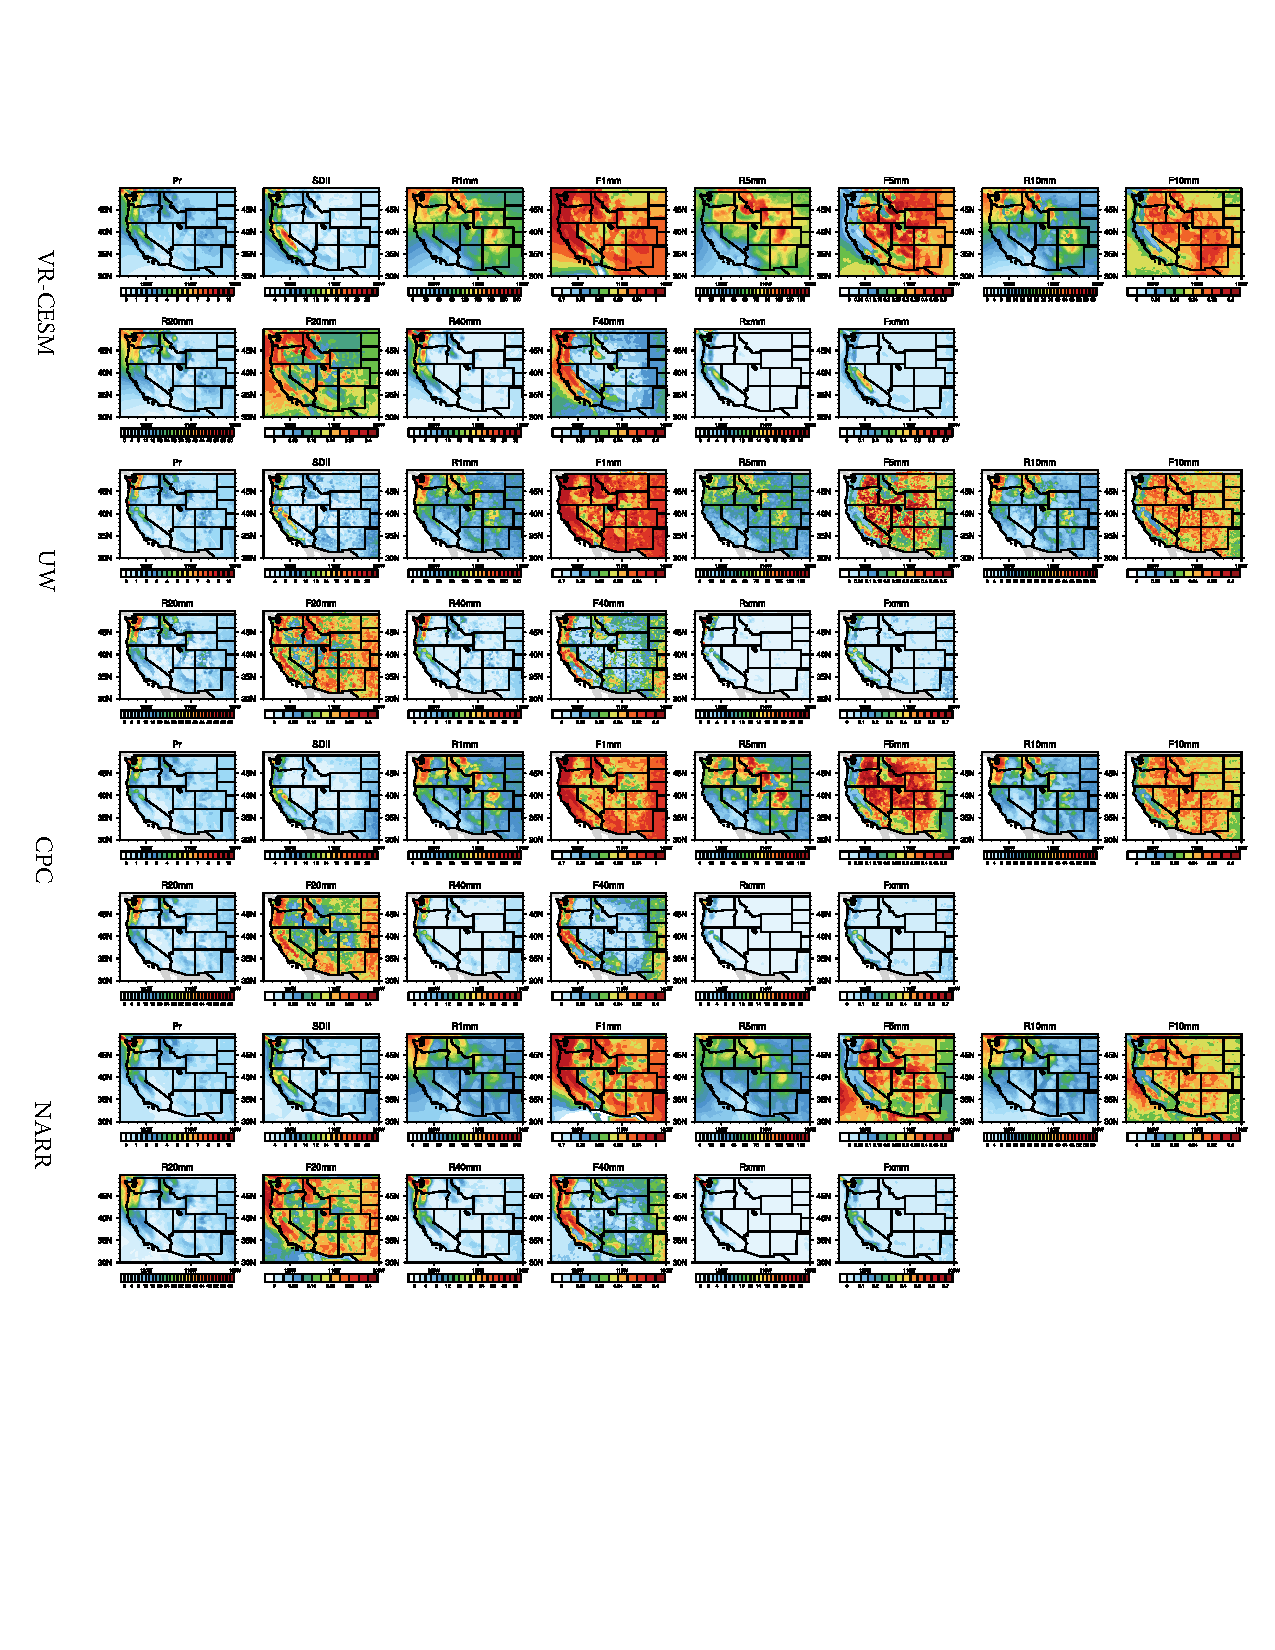
\includegraphics[width=6in]{wd_index_Hist_ref_annual_v2.pdf}
\caption{The mean precipitation and other related indices from VR-CESM and reference datasets over 1980-2005.}
\label{fig:Figure 2}
\end{center}
\end{figure}

(add fraction in this figure)

%Figure 3
\begin{figure}
\begin{center}
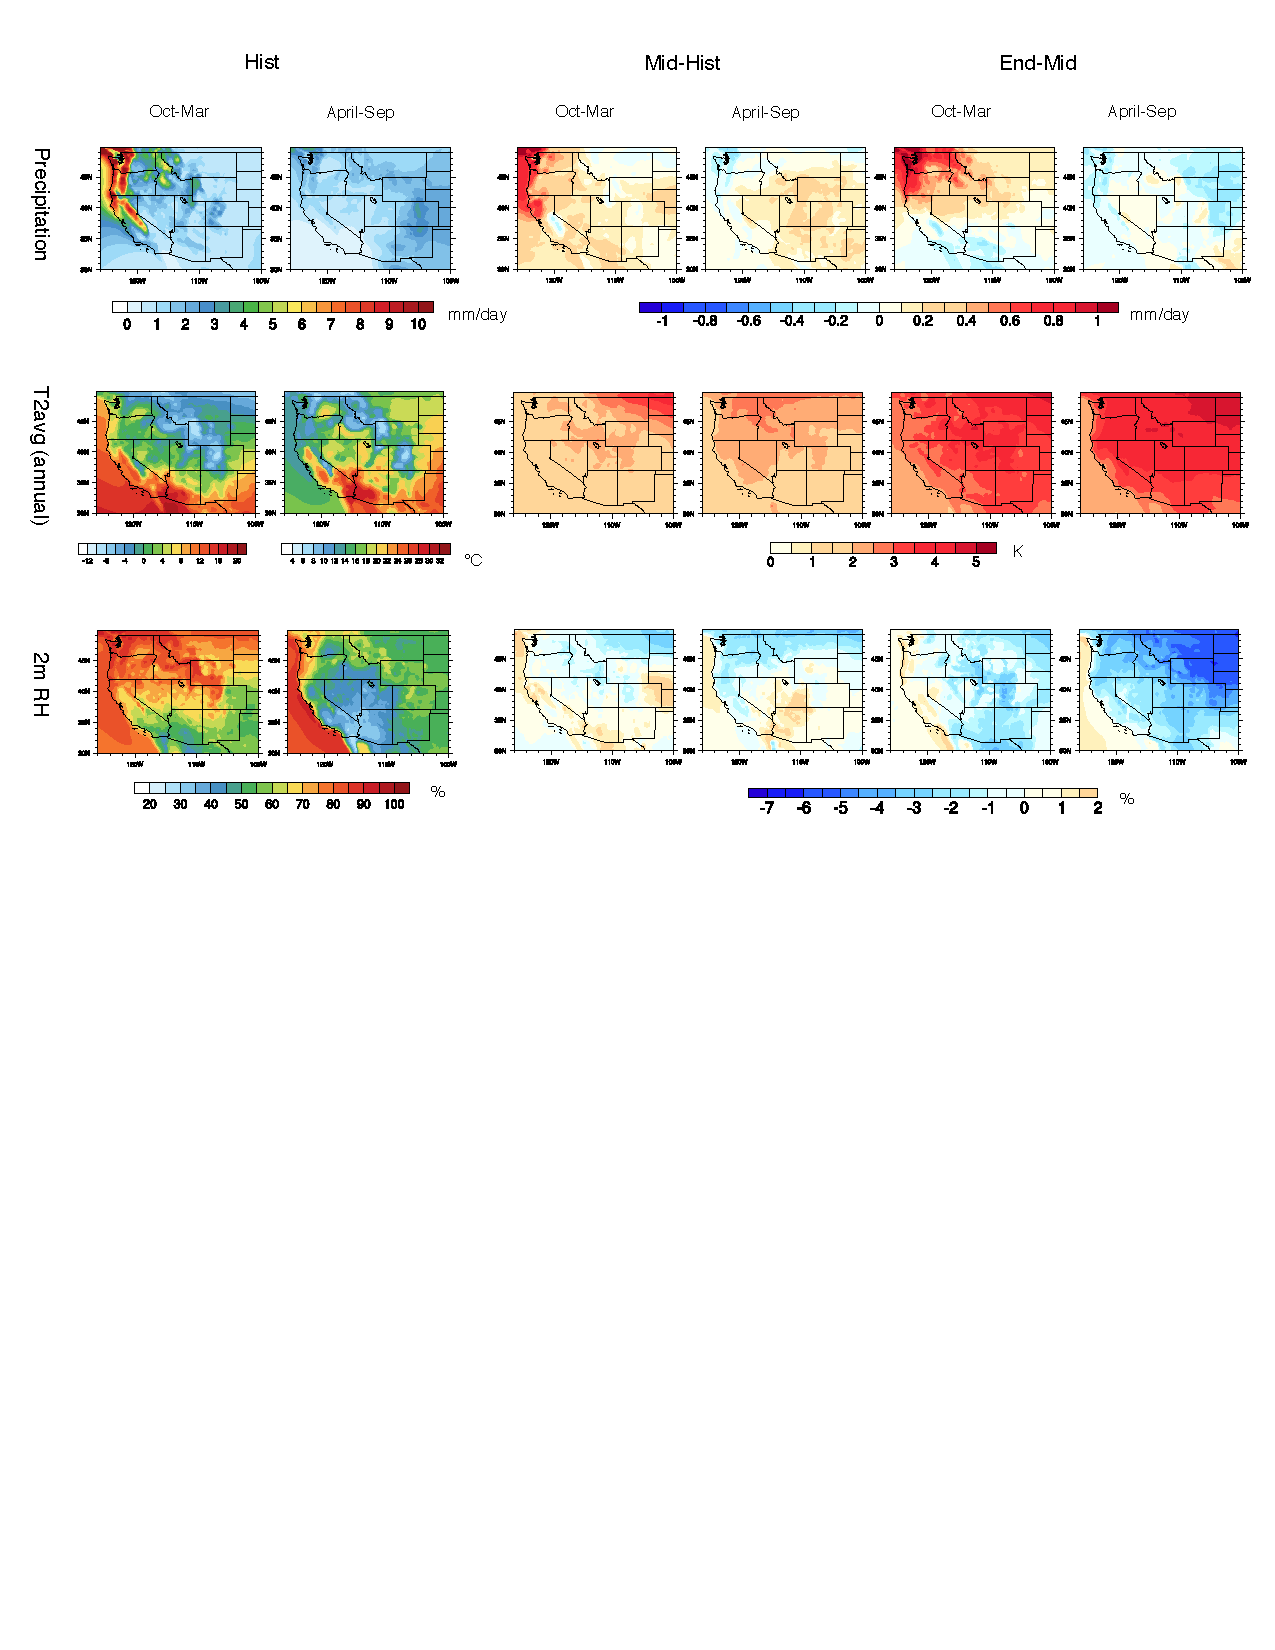
\includegraphics[width=6in]{pr_mean_clm.pdf}
\caption{The mean precipitation (Pr), 2m average temperature (T2avg), and 2m relative humidity (RH) averaged over each time period.}
\label{fig:Figure 3}
\end{center}
\end{figure}

%Figure 4
\begin{figure}
\begin{center}
\includegraphics[width=6in]{wd_index_all_years.pdf}
\caption{Differences of precipitation behaviors from past to future over western U.S. averaged over each time period.}
\label{fig:Figure 4}
\end{center}
\end{figure}

%Figure 5
\begin{figure}
\begin{center}
\includegraphics[width=6in]{wd_index_enso_wetSeason.pdf}
\caption{Difference of precipitation behaviors between warm and cool phases of ENSO from past to future over western U.S. averaged over each time period.}
\label{fig:Figure 5}
\end{center}
\end{figure}


%Figure 6
\begin{figure}
\begin{center}
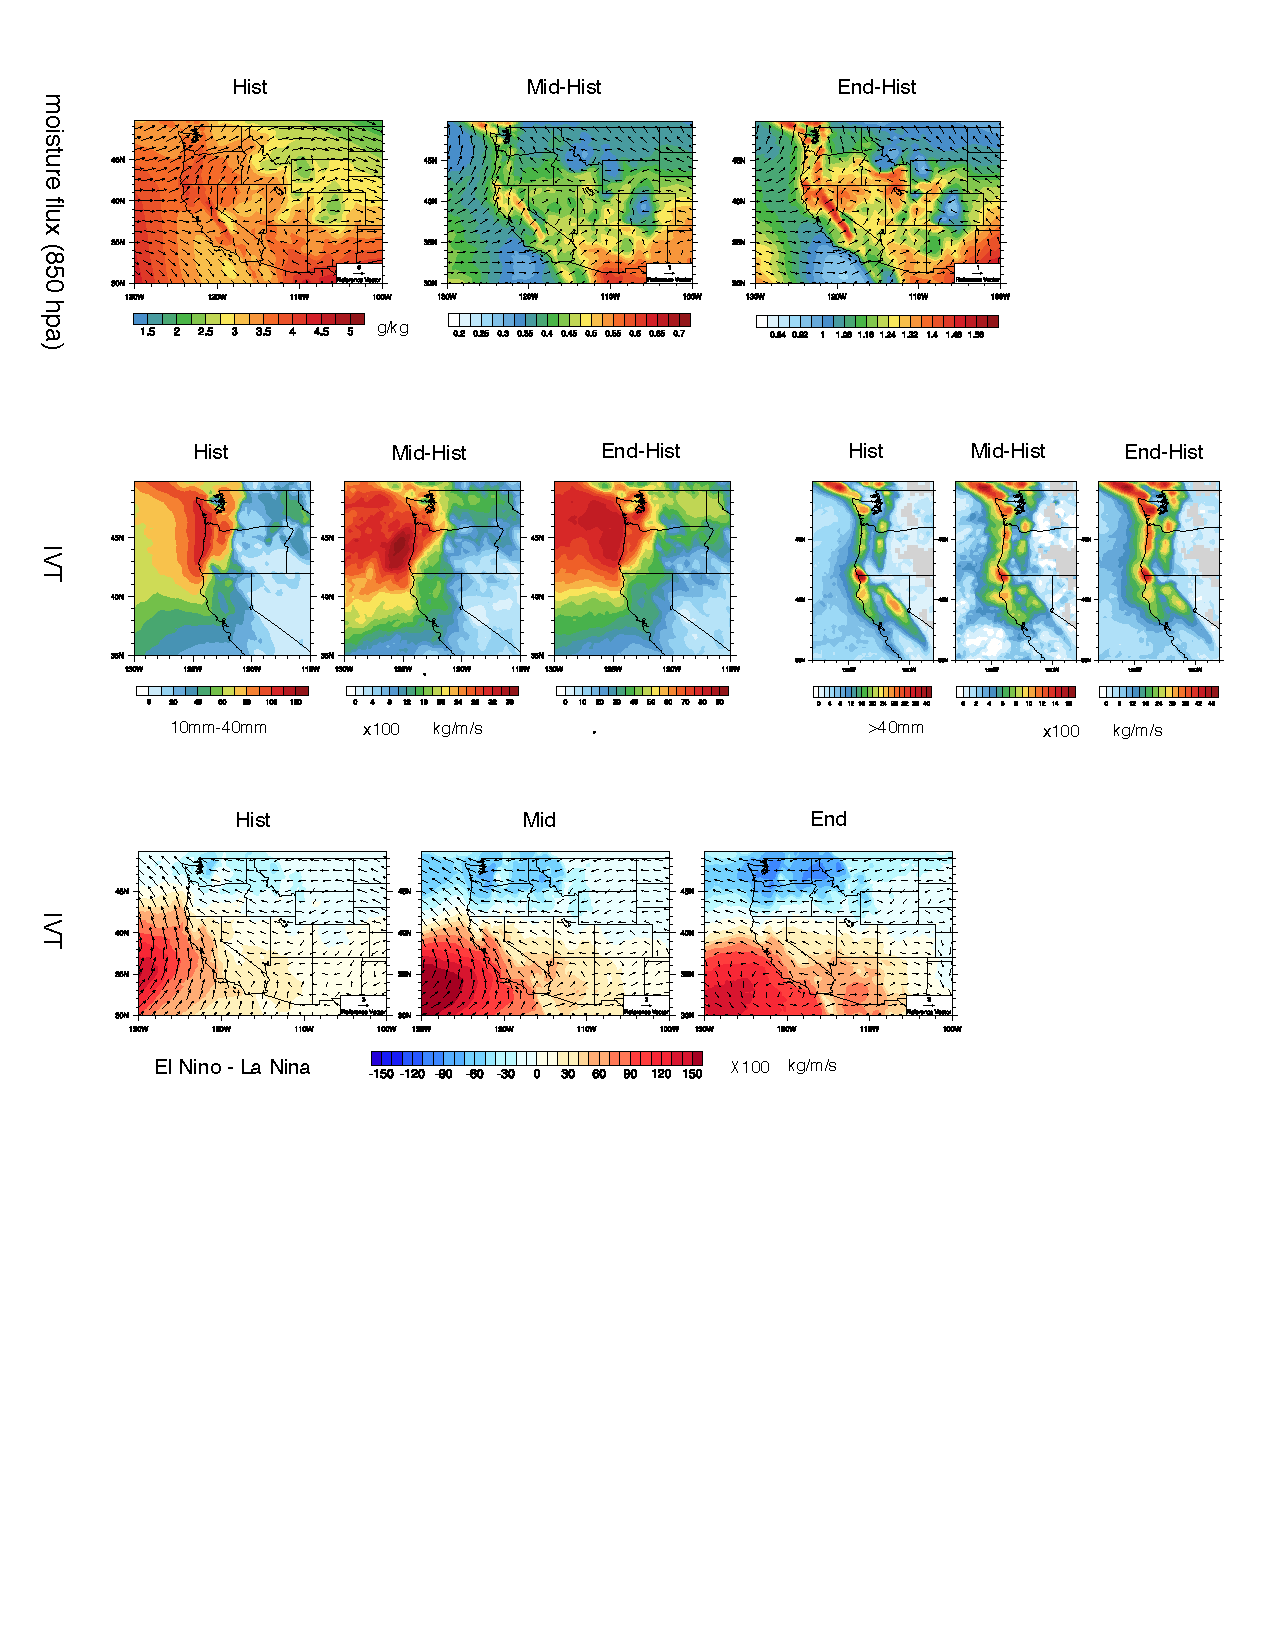
\includegraphics[width=6in]{discussion.pdf}
\caption{Changes of moisture flux at 850hPa, IVT and IWV for simulations under different time period and different phases of ENSO.}
\label{fig:Figure 6}
\end{center}
\end{figure}

(update the figure, separate the IVT and IWV for non-extreme precipitation days and extreme precipitation ones)


\end{document}
